
Lielo teksta korpusu un mašīnmācīšanās modeļu precizitātes vēsture ir cieši saistīta. Agrīnie mašīnmācīšanās algoritmi balstījās uz nelielām manuāli veidotām datu kopām, kas ierobežoja to efektivitāti. Viens no pirmajiem korpusiem bija \textit{Standard Sample of Present-Day American English}, plašāk pazīstams kā \textit{The Brown Corpus}, kas tika izdots 1964-1965. gadā un sastāvēja no apmēram viena miljona vārdu angļu teksta no dažādiem avotiem \cite{brown-corpus}, tas ir mazs apjoms teksta salīdzinot ar mūsdienās pieejamo.

Procesoru jaudas palielināšanās kopā ar datoru un interneta savienojuma pieejamību plašākai sabiedrībai ir radījuši labvēlīgu vidi izveidot un uzglabāt lielu daudzumu digitālo datu, tostarp teksta formā. Lieliem teksta korpusiem ir bijusi izšķiroša loma efektīvu mašīnmācīšanās modeļu izstrādē. Mašīnmācīšanās modeļu efektivitāte ir proporcionāla tiem pieejamo apmācības datu lielumam un kvalitātei. %source

Pirms lielu teksta korpusu pieejamības mašīnmācīšanās modeļi aprobežojās ar mazām un salīdzinoši vienkāršām datu kopām, tādēļ bija grūti sasniegt augstu precizitāti dabiskās valodas apstrādes uzdevumos. Mūsdienās lielos teksta korpusos kā Common Crawl un Wikipedia ir miljardiem vārdu vairākās valodās, kas ļauj modeļiem iemācīties ģenerēt cilvēkiem līdzīgu valodu.

Taču vai visas valodas ir līdzvērtīgi pārstāvētas korpusos? Viegli iztēloties, ka tādi lielie korpusi kā Common Crawl (kopš 2008. gada ievākti petabaiti datu no interneta mājaslapām, tostarp Vikipēdijas un Reddit) līdzvērtīgi pārstāv visu Zemes iedzīvotāju valodas. Taču valodu reprezentācija korpusos ir saistīta ar rakstītā teksta datu pieejamību šajā valodā, un neprecīzi atspoguļo cilvēku skaitu, kuri runā šajā valodā. Piemēram, valodai, kurā runā liels skaits cilvēku, korpusā var būt maz marķieru, ja šajā valodā ir maz digitāli pieejama rakstīta teksta.

Tomēr dažādi faktori traucē visiem rakstīt tekstus internetā, kas vēlāk nokļūst korpusos, piemēram, rakstītneprasme, nabadzība, ierīču un interneta nepieejamība, karš utml. Tā rezultātā korpusos ir disproporcionāli pārstāvēti gados jaunāku lietotāju no attīstītajām valstīm drukāti teksti, piemēram, GPT-2 apmācības dati tika ievākti no Reddit, un pēc Pew Internet Research pētījuma 67\% Reddit lietotāju Amerikas Savienotajās Valstīs ir vīrieši un 64\% vecumā no 18 līdz 29 gadiem.\cite{bender2021}.

Līdzīgi 87\% Vikipēdijas ierakstu veicēji ir vīrieši. Gandrīz puse dzīvo Eiropā un viena piektā daļa Ziemeļamerikā, salīdzinot ar 9.7\% un 4.8\% pasaules iedzīvotāju \cite{wikimedia2020}. Analizējot labojumus Vikipēdijas rakstos no 2001. līdz 2010. gadam, 1\% visbiežākie ierakstu veicēji uzrakstīja 77\% satura \cite{1percent}.

Korpusos tam ir vairākas praktiskas implikācijas gan sintaksē, gan semantikā. Piemēram, Vikipēdijas autors Brians Hendersons (\textit{Bryan Henderson}) 15 gados veica 90 tūkstošus labojumu, kur lielākā daļa izmaiņu ir no "comprised of" uz "comprised", kaut gan abas formas tiek pieņemtas un citos rakstiskos avotos "comprised of" ir izplatītāks (\ref{fig:distributed-representation} attēls). Tāpat BERT biežāk asociē cilvēkus ar invaliditāti ar negatīva sentimenta vārdiem un vairāki darbi to sasaista ar treniņu datu kopu īpašībām \cite{bender2021}. Pētīt negatīvu sentimentu valodu korpusos ir svarīgi, jo kompānijas reputācija ciestu, virtuālajam asistentam sniedzot atbildes ar negatīviem steriotipiem klientu apkalpošanas jomā.


\begin{figure}[h]
    \centering
    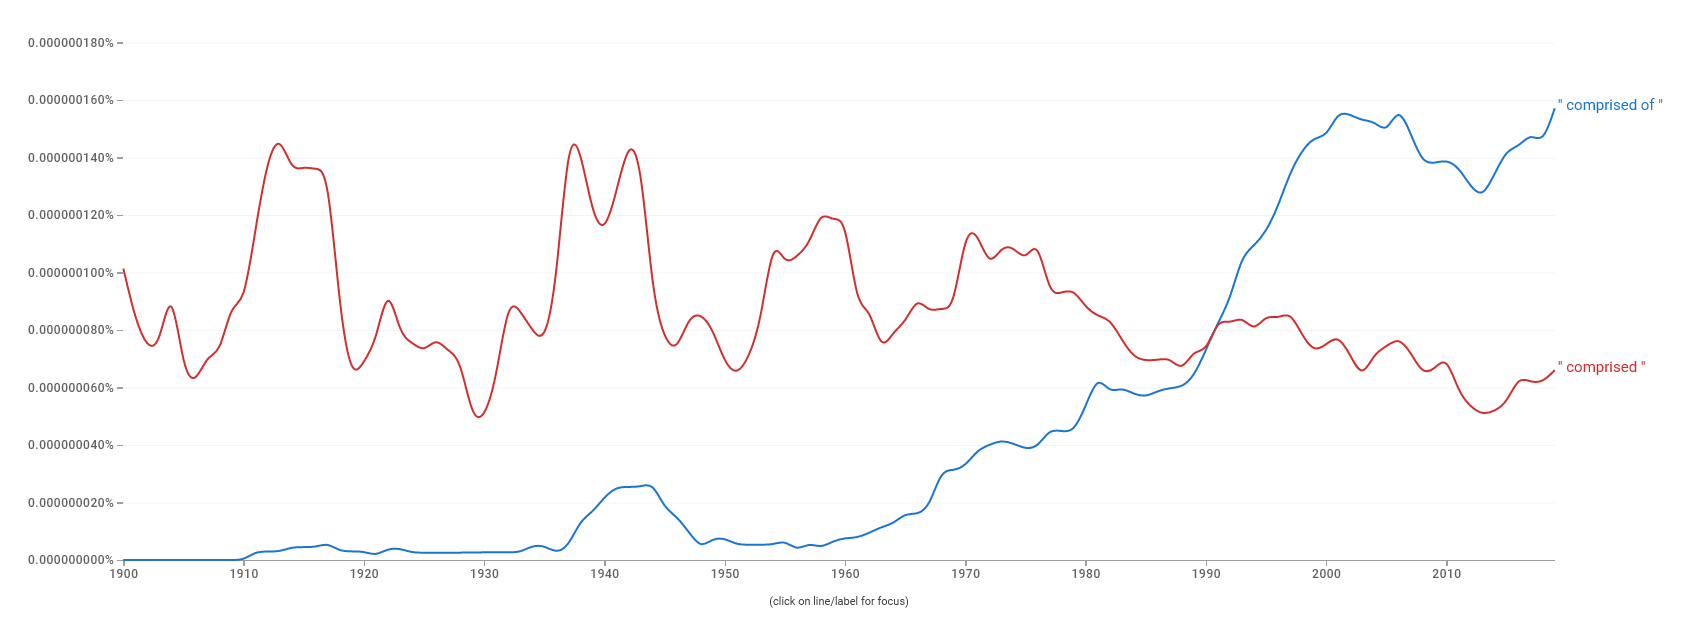
\includegraphics[width=\textwidth]{figures/comprised.png}
    \caption{Uz x ass attēloti gadi, uz y ass -- cik procentu no visiem vārdiem, kas ietverti angļu valodā rakstīto grāmatu korpusā (English 2019), ir "comprised of" un "comprised"? \cite{ngram-viewer}}
    \label{fig:comprised}
\end{figure}

Ar to tiek pierādīts, ka tekstu nav radījuši nejauši izvēlēta izlase cilvēku, tāpēc teksts nav neitrāls. Tiek paredzēts, ka virtuālos asistentus izmantos plašāks cilvēku loks nekā šobrīd internetā publicēto tekstu autori, tāpēc ir svarīgi, lai treniņdatos ir atbilstoši pārstāvēta potenciālo lietotāju valoda.


Latviešu marķieru daļa Common Crawl 100 korpusā ir atkarīga no daudziem faktoriem, tostarp latviešu satura daudzuma tīmeklī un korpusa konstruēšanā izmantotās izlases metodikas. Iespējams, ka latviešu teksta saturs korpusā ir pārāk vai nepietiekami pārstāvēts, salīdzinot ar tā izplatību tīmeklī vai proporcionāli latviešu valodā runājošo īpatsvaram.


Kas padara valodu par maz-resursu? Mazāks skaits vārdu un teikumu datu kopās, tātad mazāks skaits tokenu uz kuriem trenēt daudzvalodu jēdzientelpu modeli. Piemēram, Common Crawl-100 korpusā, uz kura trenēts XLM-R modelis, svahili un urdu valodās ir 275M un 730M tokenu attiecīgi, darbā izmantotajās - lietuviešu, latviešu, igauņu - ir 1835M, 1198M un 843M tokenu attiecīgi (\ref{tab:cc-100} tabula), tātad šīs datukopas kontekstā tās var uzskatīt par maz-resursu.


% Table generated by Excel2LaTeX from sheet 'cc-100'
\begin{table}[htbp]
    \centering
    \caption{Common Crawl-100 valodas un statistika: valodu saraksts ar marķieru (\textit{tokens}) skaitu (miljonos) un datu izmēru gibibaitos (GiB) katrai valodai}
    \begin{tabular}{llrr}
        \toprule
        ISO kods & Valoda     & Marķieri (M) & Izmērs (GiB) \\\midrule
        en       & angļu      & 55608        & 300.8        \\
        ru       & krievu     & 23408        & 278.0        \\
        lt       & lietuviešu & 1835         & 13.7         \\
        lv       & latviešu   & 1198         & 8.8          \\
        et       & igauņu     & 843          & 6.1          \\
        ur       & urdu       & 730          & 5.7          \\
        sw       & svahili    & 275          & 1.6          \\\bottomrule
    \end{tabular}
    \label{tab:cc-100}
\end{table}

\begin{figure}[h]
    \centering
    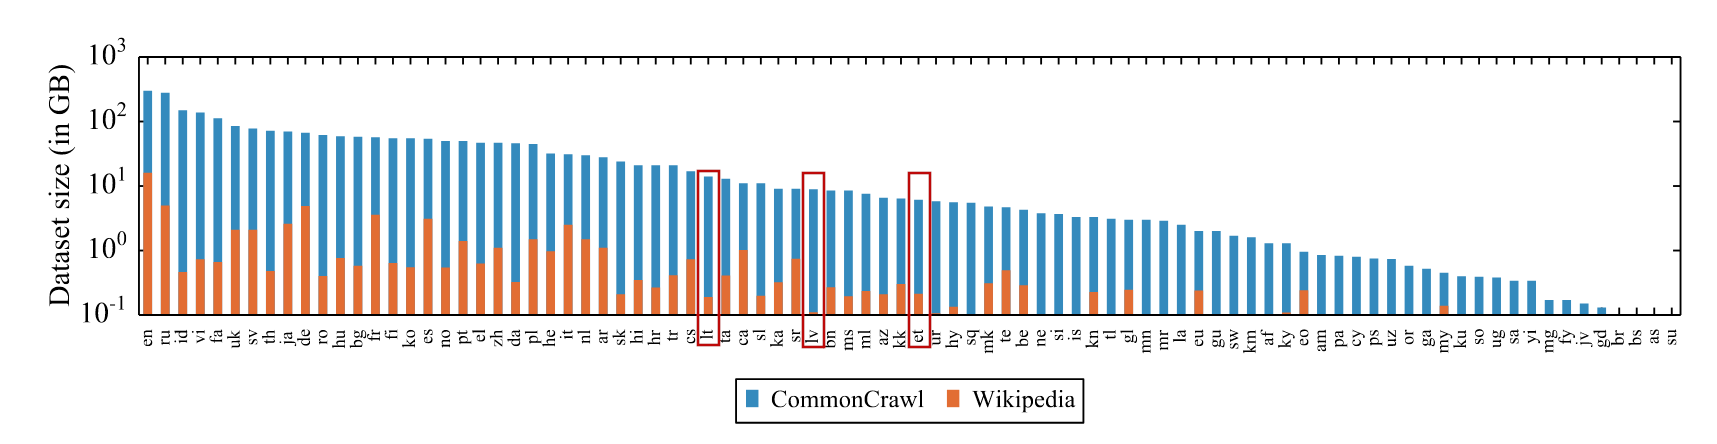
\includegraphics[width=\textwidth]{figures/dataset-size.png}
    \caption{Datu apjoms GiB (logaritmiskā skalā) valodām Wiki-100 korpusā, ko izmanto mBERT un XLM-100, un Common Crawl-100, ko izmanto XLM-R. Common Crawl-100 palielina datu apjomu par vairākām kārtām, jo īpaši maz-resursu valodās (lietuviešu, latviešu, igauņu valodas ar sarkanu izdalīju es) \cite{conneau2020}}
    \label{fig:dataset-size}
\end{figure}




% nlu korpusu part


Viens no svarīgākajiem korpusiem tieši nodomu noteikšanā ir aviokompāniju ceļojumu informācijas sistēmu (ATIS -- \textit{Airline Travel Information Systems}) datu kopa. Tā ir audioierakstu un manuālu transkriptu datu kopa, kas sastāv no cilvēku sarunām ar automatizētām aviolīniju ceļojumu informācijas sistēmām. ATIS datu kopa nodrošina lielu ziņojumu un ar tiem saistīto nodomu skaitu, ko plaši izmanto kā novērtējuma (\textit{benchmark}) datu kopu klasifikatoru apmācībai nodomu noteikšanā \cite{atis1990}.


SNIPS -- \textit{Spoken Natural Language Interaction for Personal Assistant}) datu kopā ir 16 000 ievadi, kas sadalīti septiņos nodomos: SearchCreativeWork, GetWeather, BookRestaurant, PlayMusic, AddToPlaylist, RateBook, SearchScreeningEvent \cite{snips-2018}.


Lietotāja dabiskās valodas ievads tiek pārveidots jēdzientelpā, un tad pēc tam klasifikators nosaka lietotāja nodomu.

Dabisko valodu saprašanas (Natural Language Understanding (NLU)) uzdevumi iedalās divās daļās: nodomu noteikšana un parametru \textit{slots}) iegūšana no ievadiem \textit{slot filling}) (\ref{tab:slots} tabula) \cite{snips-2018}. Šajā darbā tiks apskatīts pirmais solis -- nodomu noteikšana.


\begin{table}[htbp]
    \centering
    \caption{``Weather" datu kopa, uz kuras tika apmācīts virtuālais asistents, kas apstrādā lietotāja vaicājumus par laikapstākļiem  \cite{snips-2018}}
    \begin{tabular}{rlr}
        Nodoms            & Parametrs                                           & Piemēri                                                                                                                                            \\
        & \textcolor[rgb]{ .439,  .188,  .627}{ region}           & Is it \textcolor[rgb]{ 1,  .753,  0}{cloudy} in \textcolor[rgb]{ 1,  0,  0}{Germany} \textcolor[rgb]{ .573,  .816,  .314}{ right now}?                         \\
        & \textcolor[rgb]{ 1,  0,  0}{ country}                   & Is \textcolor[rgb]{ .439,  .188,  .627}{South Carolina} expected to be \textcolor[rgb]{ 1,  .753,  0}{sunny} \textcolor[rgb]{ .573,  .816,  .314}{in 2 hours}? \\
        ForecastCondition & \textcolor[rgb]{ .573,  .816,  .314}{ datetime}         & Is there \textcolor[rgb]{ 1,  .753,  0}{snow} in \textcolor[rgb]{ 0,  .69,  .941}{Paris}?                                                                  \\
        & \textcolor[rgb]{ 0,  .69,  .941}{ locality}             & Should I expect a \textcolor[rgb]{ 1,  .753,  0}{storm} near \textcolor[rgb]{ .929,  .49,  .192}{Mount Rushmore}?                                          \\
        & \textcolor[rgb]{ 1,  .753,  0}{ condition}              &                                                                                                                                                    \\
        & \textcolor[rgb]{ .929,  .49,  .192}{ point of interest} &                                                                                                                                                    \\
    \end{tabular}%
    \label{tab:slots}%
\end{table}%


Korpusi ir paredzēti izmantošanai dabiskās valodas izpratnes uzdevumiem -- nodomu noteikšanai un entītiju atpazīšanai.

Ask Ubuntu korpuss sastāv no 162 jautājumiem un atbildēm, kas iegūti vietnē \url{https://askubuntu.com}. Šis korpuss ir anotēts ar pieciem dažādiem nolūkiem: MakeUpdate, SetupPrinter, ShutdownComputer, SoftwareRecommendation un None. Papildus šiem nolūkiem korpusā ir iekļauti arī trīs entītiju veidi: printeris, programmatūra un versija, tomēr entītiju noteikšana ir ārpus šī darba tvēruma \textit{scope}) \cite{braun-2017}. Pateicoties konkrētiem nodomiem un entītiju veidiem, izstrādātāji var koncentrēties uz precīzāku modeļu izveidi konkrētiem uzdevumiem, piemēram, printera iestatīšanai vai programmatūras atjaunināšanai.

Ask Ubuntu korpuss ir noderīgs resurss Ubuntu un citu Linux operētājsistēmu lietotāju pieredzes uzlabošanai. Tā kā Ubuntu ir pieejams daudzās valodās virutālā asistenta spēja atbildēt uz Ubuntu jautājumiem lietotāja izvēlētajā valodā var ievērojami palielināt operētājsistēmas pieejamību un lietojamību. Piemēram, trenējot virtuālos asistentus uz šī korpusa izstrādātāji var izveidot lietotājiem draudzīgas saskarnes \textit{interfaces}). 


Tīmekļa lietojumprogrammu korpuss (\textit{Web Applications Corpus}), turpmāk "webapps" korpuss ir vērtīgs resurss virtuālo asistentu izstrādei, kas var palīdzēt lietotājiem orientēties un novērst ar tīmekļa lietojumprogrammām saistītas problēmas. Ar 89 jautājumiem un atbildēm, kas iegūtas vietnē \url{https://webapps.stackexchange.com}, šis korpuss aptver dažādas tēmas un scenārijus, ar kuriem lietotāji var saskarties, izmantojot tīmekļa lietojumprogrammas. Korpusam ir astoņas anotācijas -- ChangePassword, DeleteAccount, DownloadVideo, ExportData, FilterSpam, FindAlternative, SyncAccounts un None --, kā arī trīs entītiju veidi: WebService, OS un Browser \cite{braun-2017}. Uz šī korpusa apmācīti mašīnmācīšanās modeļi var noteikt lietotāju nodomus un sniegt atbildes, tādā veidā uzlabojot lietotāja pieredzi ar tīmekļa lietojumprogrammām.



Chatbot korpuss tika iegūts no Telegram virtuālā asistenta Minhenes sabiedriskajam transportam. Tas satur 206 jautājumus, kas tika anotēti divos nolūkos -- DepartureTime un FindConnection --, kā arī piecus entītiju veidus: StationStart, StationDest, Criterion, Vehicle un Line \cite{braun-2017}. Šis korpuss ir īpaši noderīgs, lai izstrādātu virtuālos asistentus, kas palīdz lietotājiem orientēties sabiedriskajā transportā, jo tas nodrošina skaidru un kodolīgu jautājumu un entītiju kopumu šajā jomā. 
